\documentclass[a4paper,11pt,uplatex]{jsarticle}


% 数式
\usepackage{amsmath,amsfonts}
\usepackage{bm}
\usepackage{physics}
% 画像
\usepackage[dvipdfmx]{graphicx}
\usepackage[dvipdfmx,colorlinks=true,linkcolor=blue]{hyperref}
\usepackage{pxjahyper}

\begin{document}


\section{考察}
\subsection{光学系}
回折パターンを決定する要素として放射光関数と光学系関数がある。
エネルギーを求めるには放射光の情報が分かれば良いが、今回は放射光関数を仮定している。
光学系関数の光学計算は原理的には正確に計算可能である
光学系によって、分光された光の情報から入射光の情報を逆演算する系を構築することができれば精度の向上につながる









\clearpage

\begin{figure}[tb]
  \centering
  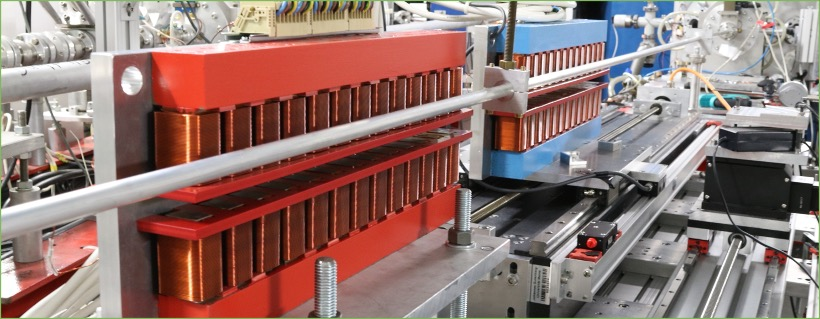
\includegraphics[width=0.8\linewidth]{image/1-1.jpg}\\
  \caption{サンプルの図}
  \label{sample_image}
\end{figure}

\begin{itemize}
  \item a
\end{itemize}
\begin{enumerate}
  \item b
\end{enumerate}

\begin{align}
\frac{1}{2} = \qty(\frac{1}{3}) + \qty{1}\Sigma
\end{align}
\end{document}